
\documentclass{article}

%% Packages for French writing
\usepackage[french]{babel}
\usepackage[utf8]{inputenc}
\usepackage[T1]{fontenc}
\usepackage{layout}

%% Packages for Math symbols
\usepackage[fleqn]{amsmath}
\usepackage{amssymb}
\usepackage{mathrsfs}

%% Packages for figures insertion
\usepackage{graphicx}
\usepackage{wrapfig}
\usepackage{framed}
\usepackage{float}

%% Package for document margin editing
\usepackage[top=2cm, bottom=2cm, left=2cm, right=2cm]{geometry}

%% Package for source code insertion
\usepackage{listings}
\usepackage{xcolor}
\definecolor{grey}{rgb}{0.97, 0.97, 0.97}
\definecolor{darkred}{rgb}{0.42, 0, 0}
\definecolor{darkblue}{rgb}{0, 0, 0.42}
\definecolor{darkgrey}{rgb}{0.22, 0.22, 0.82}
\definecolor{green}{HTML}{088A08}
\lstset{
  basicstyle=\small\sffamily\footnotesize,
  captionpos=b,
  numbers=left,
  numberstyle=\tiny,
  tabsize=4,
  frame=trBL,
  backgroundcolor=\color{grey},
  commentstyle=\color{green},
  keywordstyle=\color{darkblue}\bf,
  identifierstyle=\color{darkgrey},
  stringstyle=\color{darkred}
}

\setlength\parindent{0pt}
\setlength\parskip{3pt}
\title{ARCHI2 - Compte-rendu du TME1}
\author{Nicolas Phan}
\date{pour le 17 Janvier 2018}
\begin{document}
\pagestyle{headings}
\maketitle
\tableofcontents
\newpage

%==================================================================================================
%=========================  Introduction  =========================================================
%==================================================================================================

%----------------- Objectif -----------------------------------------------------------------------

\section{Automate du composant PibusSimpleRam}

\subsection{Machine à états du composant}

\begin{figure}[H]
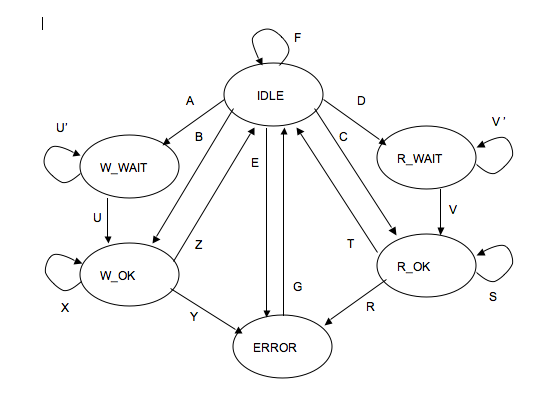
\includegraphics[width=0.75\textwidth]{pics/mae_ram.png}
\centering
\caption{Graphe de la MAE du composant RAM}
\label{mae_ram}
\end{figure}

\begin{table}[H]
\centering
\begingroup
\setlength{\tabcolsep}{5pt}
\renewcommand{\arraystretch}{1.1}
\begin{tabular}{ | c | l | }
\hline
Fonction    &   Transition  \\
\hline
\texttt{A}  &   \tt{SEL.ADR\_OK.$\overline{\tt{READ}}$.DELAY                     }\\
\texttt{B}  &   \tt{SEL.ADR\_OK.$\overline{\tt{READ}}$.$\overline{\tt{DELAY}}$        }\\
\texttt{C}  &   \tt{SEL.ADR\_OK.READ.$\overline{\tt{DELAY}}$                     }\\
\texttt{D}  &   \tt{SEL.ADR\_OK.READ.DELAY                                  }\\
\texttt{E}  &   \tt{SEL.$\overline{\tt{ADR\_OK}}$                                }\\
\texttt{F}  &   \tt{$\overline{\tt{SEL}}$                                        }\\
\texttt{G}  &   \tt{1                                                       }\\
\hline
\texttt{U}  &   \tt{$\overline{\tt{GO}}$                                         }\\
\texttt{U'} &   \tt{GO                                                      }\\
\hline
\texttt{V}  &   \tt{$\overline{\tt{GO}}$                                         }\\
\texttt{V'} &   \tt{GO                                                      }\\
\hline
\texttt{X}  &   \tt{SEL.ADR\_OK.$\overline{\tt{READ}}$                           }\\
\texttt{Y}  &   \tt{SEL.($\overline{\tt{ADR\_OK}}$ + READ)                       }\\
\texttt{Z}  &   \tt{$\overline{\tt{SEL}}$                                        }\\
\hline
\texttt{R}  &   \tt{SEL.($\overline{\tt{ADR\_OK}}$ + $\overline{\tt{READ}}$)          }\\
\texttt{S}  &   \tt{SEL.ADR\_OK.READ                                        }\\
\texttt{T}  &   \tt{$\overline{\tt{SEL}}$                                        }\\
\hline
\end{tabular}
\endgroup
\caption{Expression des fonctions de transitions de la MAE du composant RAM}
\label{standard}
\end{table}

\begin{table}[H]
\centering
\begingroup
\setlength{\tabcolsep}{5pt}
\renewcommand{\arraystretch}{1.1}
\begin{tabular}{| l | l | l | l | l |}
\hline
                    & \tt{ACK\_EN}      & \tt{ACK\_VALUE}   & \tt{DT\_EN} & \tt{MEM\_CMD}   \\
\hline
\tt{IDLE}           & \tt{0}            & \tt{WAIT}         & \tt{0}      & \tt{NOPE}         \\
\tt{R\_WAIT}        & \tt{1}            & \tt{WAIT}         & \tt{0}      & \tt{READ}         \\
\tt{R\_OK}          & \tt{1}            & \tt{READY}        & \tt{0}      & \tt{READ}         \\
\tt{W\_WAIT}        & \tt{1}            & \tt{WAIT}         & \tt{1}      & \tt{WRITE}        \\
\tt{W\_OK}          & \tt{1}            & \tt{READY}        & \tt{1}      & \tt{WRITE}        \\
\tt{ERROR}          & \tt{1}            & \tt{ERROR}        & \tt{0}      & \tt{NOPE}         \\
\hline
\end{tabular}
\endgroup
\caption{Expression des fonctions de transitions de la MAE du composant RAM}
\label{standard}
\end{table}







\begin{enumerate}
\item \textbf{Modélisation}  : Cela consiste en la description d'un modèle du processeur,
\end{enumerate}

La Figure \ref{outils} résume le flot de travail et les outils utilisés pour les étapes de Syntèse,
Placement et Routage.

\begin{eqnarray*}
  \sum_{\substack{k \in [[0, 4]] \\ \texttt{shift\_value(k)} = 1}} 2^k &= \texttt{shift\_value}
\end{eqnarray*}

%code : les xxx_t
%\lstinputlisting[language=vhdl, firstline=560, lastline=579]{decod.vhdl}

%==================================================================================================
%=========================  End of the Document  ==================================================
%==================================================================================================

\end{document}
